\chapter{Batteries, Fuel Cells and Electrolysis}\label{ch:b2:batteries-electrolysis}

Every kilogram of aluminium won from its ore takes about \qty{13}{kW.h} of
electricity; melting down a kilogram of scrap takes, in principle, the
\qty{0.3}{kW.h} that heats it to its melting point and melts it. The difference
is the work of a long row of \omterm{def:b2:batteries-electrolysis:electrolysis}{electrolysis} cells, each passing hundreds of
thousands of amperes through molten salt at a few volts. A battery runs the
other way: a spontaneous reaction drives the current. With the
\omterm{def:b2:current-potential-curves:ie-curve}{current--potential curves} of \cref{ch:b2:current-potential-curves}, both are
read on the same diagram, and so is a piece of zinc dissolving in acid.
% ledger: hT:Al_l.933, aw:Al

\begin{recall}
\Cref{ch:b2:cell-thermodynamics}: $\Delta_r G = -nFE$, maximum work, the
\omterm{def:b2:cell-thermodynamics:faraday}{Faraday constant}. \Cref{ch:b2:current-potential-curves}: \omterm{def:b2:current-potential-curves:ie-curve}{current--potential
curves}, fast and \omterm{def:b2:current-potential-curves:fast-slow}{slow systems}, \omterm{def:b2:current-potential-curves:overpotential}{overpotentials}, \omterm{def:b2:current-potential-curves:limiting-current}{limiting currents}, the walls of
water. \Cref{ch:b2:ellingham}: why aluminium is not won by carbon. The school
volume: \omterm{def:b2:batteries-electrolysis:electrolysis}{electrolysis}, \omterm{def:b2:batteries-electrolysis:battery}{accumulators}.
\end{recall}

\begin{omfigure}
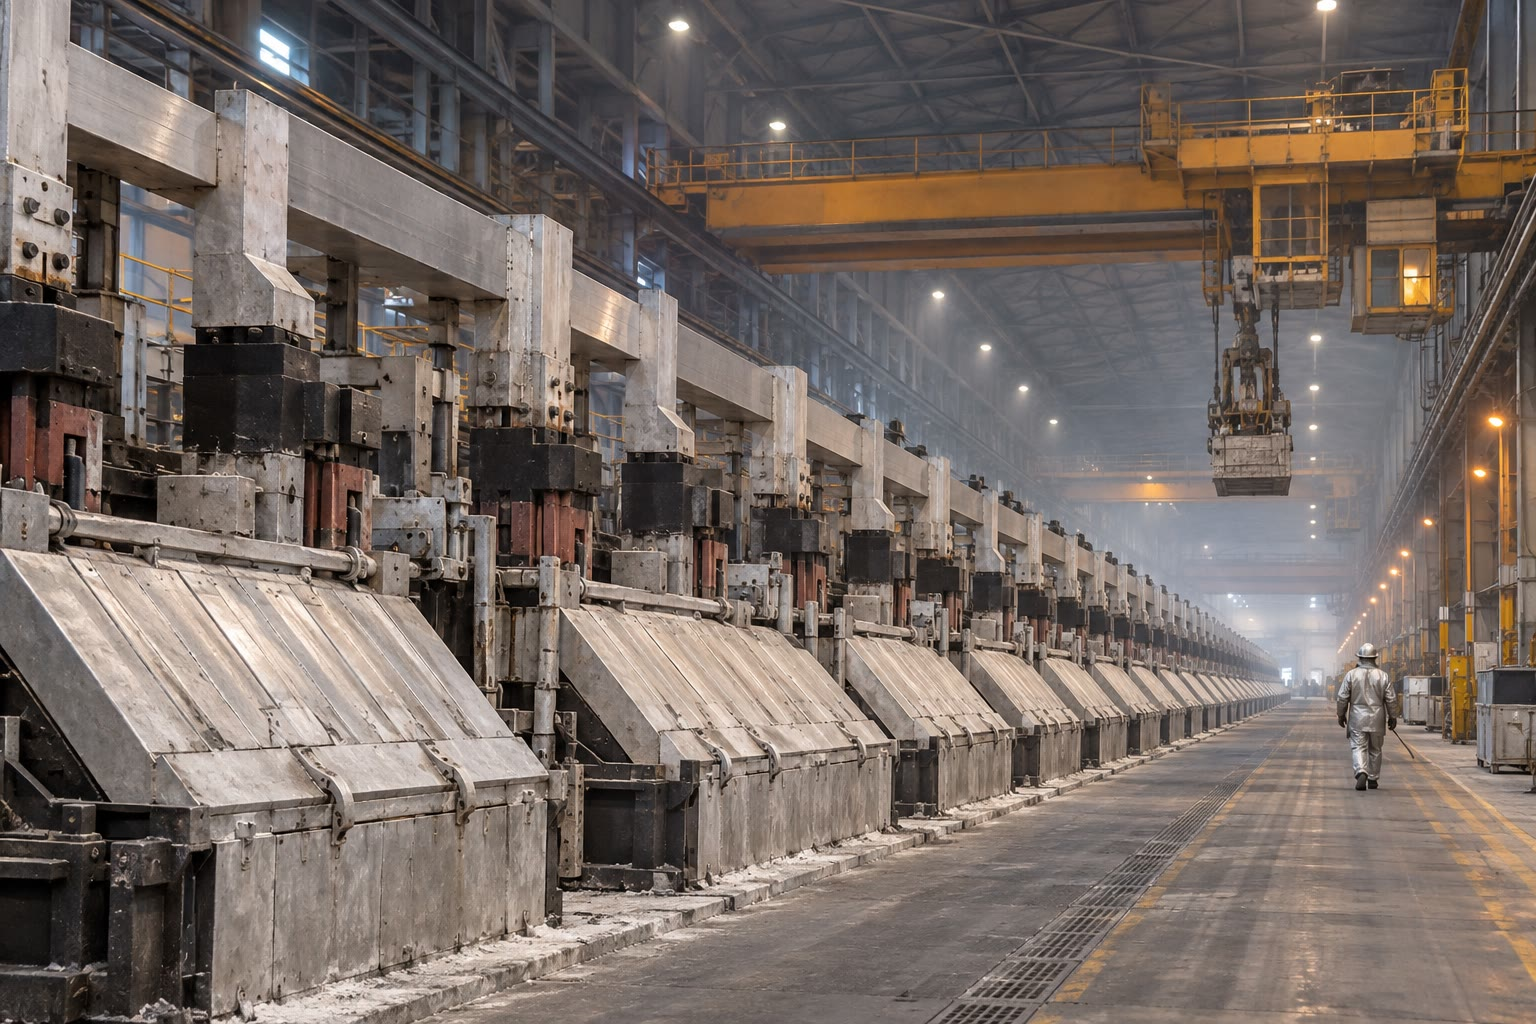
\includegraphics[width=0.62\linewidth]{images/book3/ai/b2-11-potroom.jpg}

{\small The potroom of an aluminium smelter: a row of \omterm{def:b2:batteries-electrolysis:electrolysis}{electrolysis} cells,
hundreds long, connected in series; the overhead crane changes the carbon
anodes as they burn away.}
\end{omfigure}

\section{Spontaneous reactions read on curves}

\begin{definition}[Mixed potential]\label{def:b2:batteries-electrolysis:mixed-potential}
The \emph{mixed potential}\index{mixed potential} of an electrode on which two
different couples react, one oxidised and one reduced, is the potential it
takes when no net current flows: the \omterm{def:b2:current-potential-curves:ie-curve}{anodic current} of one couple is then
equal and opposite to the \omterm{def:b2:current-potential-curves:ie-curve}{cathodic current} of the other.
\end{definition}

\begin{proposition}[A metal in a solution]\label{prop:b2:batteries-electrolysis:mixed}
A metal dipping into a solution that can oxidise it settles at the potential
$E_m$ where $i_a(E_m) = -i_c(E_m)$, the \omterm{def:b2:current-potential-curves:ie-curve}{anodic current} of the metal's
oxidation balancing the \omterm{def:b2:current-potential-curves:ie-curve}{cathodic current} of the oxidant's reduction; the
metal dissolves at the rate $i_a(E_m)/(nF)$.
\end{proposition}

\begin{proof}
An isolated piece of metal carries no net current. Both half-reactions happen
on its surface at the same potential, so their currents, read on their curves
at that potential, add up to zero. By \cref{prop:b2:current-potential-curves:current-rate},
the \omterm{def:b2:current-potential-curves:ie-curve}{anodic current} gives the rate of oxidation.
\end{proof}

\begin{omfigure}
\begin{tikzpicture}
\begin{axis}[omie, width=0.82\linewidth, height=6cm, xmin=-1.1, xmax=-0.3,
  ymin=-3, ymax=3, xlabel={$E$ (V)}, ylabel={$i$}, clip=true, clip mode=individual,
  axis y line=left]
\addplot[omanodic] table[x=E, y=i] {figdata/out/bachelor-2-ie-curves-f-Zn.dat};
\addplot[omcathodic] table[x=E, y=i] {figdata/out/bachelor-2-ie-curves-f-HZn.dat};
\addplot[omcathodic, dashed] table[x=E, y=i] {figdata/out/bachelor-2-ie-curves-f-HCu.dat};
\draw[densely dotted] (axis cs:-0.820,-0.148) -- (axis cs:-0.820,0.148);
\draw[densely dotted] (axis cs:-0.737,-2.38) -- (axis cs:-0.737,2.38);
\fill (axis cs:-0.820,0.148) circle (1.3pt); \fill (axis cs:-0.737,2.38) circle (1.3pt);
\node[font=\scriptsize, anchor=south east] at (axis cs:-0.825,0.2) {zinc alone};
\node[font=\scriptsize, anchor=west] at (axis cs:-0.73,2.38) {zinc touching copper};
\node[font=\scriptsize, omThm, anchor=west] at (axis cs:-0.70,1.2) {\ce{Zn} $\to$ \ce{Zn^2+}};
\node[font=\scriptsize, omDef, anchor=north west, align=left] at (axis cs:-0.87,-0.5) {\ce{H+} $\to$ \ce{H2}\\ on zinc};
\node[font=\scriptsize, omDef, anchor=north west] at (axis cs:-0.66,-1.7) {on copper};
\end{axis}
\end{tikzpicture}

{\small Zinc in acid (model curves, zinc ions dilute; potentials from
$-1.1$ to \qty{-0.3}{V}). Alone, zinc settles at
the \omterm{def:b2:batteries-electrolysis:mixed-potential}{mixed potential} where its oxidation balances the slow reduction of
\ce{H+} on zinc: a small current, a slow dissolution. Touching copper, on which
the reduction of \ce{H+} is less slow, the balance moves to a higher potential
and a current more than ten times larger: the zinc dissolves fast, hydrogen
bubbles on the copper.}
\end{omfigure}

The same reading explains corrosion (\cref{ch:b2:corrosion}): the corrosion
rate of a metal is the current at its \omterm{def:b2:batteries-electrolysis:mixed-potential}{mixed potential}.

\section{Cells delivering a current}

\begin{definition}[Batteries]\label{def:b2:batteries-electrolysis:battery}
A \emph{primary cell}\index{primary cell} is an electrochemical cell used
once, until its reagents are spent. An \emph{accumulator}\index{accumulator}
is a cell that can be recharged by forcing a current through it in the
reverse direction, which reverses its reaction. The \emph{specific
energy}\index{specific energy} of a cell is the electrical energy it delivers
per unit mass, usually in \unit{W.h/kg}.
\end{definition}

\begin{proposition}[Voltage of a cell delivering a current]\label{prop:b2:batteries-electrolysis:delivering}
A cell delivering a current $I$ has a voltage
\[
  U = E_+ - E_- - \eta_a - |\eta_c| - rI ,
\]
where $E_+$ and $E_-$ are the equilibrium potentials of its two electrodes,
$\eta_a > 0$ the \omterm{def:b2:current-potential-curves:overpotential}{overpotential} of the oxidation at the negative electrode,
$\eta_c < 0$ that of the reduction at the positive electrode, and $r$ the
internal resistance (electrolyte, separator, connections).
\end{proposition}

\begin{proof}
The same current $I$ is anodic at the negative electrode, whose potential is
read on its anodic curve, $E_- + \eta_a$, and cathodic at the positive one,
whose potential is $E_+ + \eta_c$. Between them the current crosses the
electrolyte, where the potential drops by $rI$. Hence $U = (E_+ + \eta_c) - (E_- +
\eta_a) - rI$.
\end{proof}

\begin{omfigure}
\begin{tikzpicture}
\begin{axis}[omie, width=0.82\linewidth, height=5.6cm, xmin=-1.2, xmax=0.8,
  ymin=-2, ymax=2, xlabel={$E$ (V)}, ylabel={$i$}, clip=true, clip mode=individual]
\addplot[omanodic] table[x=E, y=i] {figdata/out/bachelor-2-ie-curves-h-neg.dat};
\addplot[omcathodic] table[x=E, y=i] {figdata/out/bachelor-2-ie-curves-h-pos.dat};
\draw[densely dashed, gray] (axis cs:-1.2,1) -- (axis cs:0.8,1);
\draw[densely dashed, gray] (axis cs:-1.2,-1) -- (axis cs:0.8,-1);
\node[font=\scriptsize, gray, anchor=south west] at (axis cs:-1.18,1) {$+I$};
\node[font=\scriptsize, gray, anchor=north west] at (axis cs:-1.18,-1) {$-I$};
\fill (axis cs:-0.730,1) circle (1.3pt); \fill (axis cs:0.210,-1) circle (1.3pt);
\draw[densely dotted] (axis cs:-0.85,0) -- (axis cs:-0.85,0.5);
\draw[densely dotted] (axis cs:0.45,0) -- (axis cs:0.45,-0.5);
\node[font=\scriptsize, anchor=south] at (axis cs:-0.85,0.5) {$E_-$};
\node[font=\scriptsize, anchor=north] at (axis cs:0.45,-0.5) {$E_+$};
\draw[<->, thick, omProp] (axis cs:-0.730,1.5) -- (axis cs:0.210,1.5) node[midway, above, font=\scriptsize] {$U + rI$};
\draw[densely dotted] (axis cs:-0.730,1) -- (axis cs:-0.730,1.5);
\draw[densely dotted] (axis cs:0.210,-1) -- (axis cs:0.210,1.5);
\node[font=\scriptsize, omThm, anchor=west] at (axis cs:-0.70,0.6) {negative electrode};
\node[font=\scriptsize, omDef, anchor=west] at (axis cs:0.30,-1.5) {positive electrode};
\end{axis}
\end{tikzpicture}

{\small The operating point of a cell (model curves). At a current $I$ the
negative electrode sits on its anodic curve, the positive electrode on its
cathodic curve; the difference of the two potentials, less the ohmic drop
$rI$, is the voltage delivered. It falls as $I$ grows.}
\end{omfigure}

\begin{method}[The operating point of a cell or an electrolyser]\label{met:b2:batteries-electrolysis:operating-point}
\begin{enumerate}
  \item Draw the anodic curve of the electrode that is oxidised and the
        cathodic curve of the one that is reduced.
  \item For a current $I$, read the potential of each electrode at $+I$ on the
        anodic curve and at $-I$ on the cathodic one.
  \item The difference of the two potentials, corrected by $rI$ (subtracted for
        a cell, added for an \omterm{def:b2:batteries-electrolysis:electrolysis}{electrolyser}), is the voltage.
\end{enumerate}
\end{method}

\begin{example}[The lead--acid accumulator]\label{ex:b2:batteries-electrolysis:lead}
At the negative electrode \ce{Pb + SO4^2- -> PbSO4 + 2e-}; at the positive one
\ce{PbO2 + 4H+ + SO4^2- + 2e- -> PbSO4 + 2H2O}. Overall
\[
  \ce{Pb + PbO2 + 4H+ + 2SO4^2- -> 2PbSO4 + 2H2O},
\]
$\Delta_r G^\circ = 2(-813.14) + 2(-237.13) - (-217.33) - 2(-744.53) =
\qty{-394.1}{kJ/mol}$, $E^\circ = 394\,100/(2 \times 96\,485) = \qty{2.04}{V}$.
Both electrodes are covered by lead sulfate as the cell discharges; charging
reverses the reaction. The reduction of \ce{H+} on lead and the oxidation of
water on lead dioxide are slow: that is why a cell of \qty{2}{V} can be charged
in water, whose thermodynamic window is only \qty{1.23}{V} wide.
% ledger: dfg:PbSO4_cr, dfg:H2O_l, dfg:PbO2_cr, dfg:SO42-_ao
\end{example}

\begin{omfigure}
\begin{tikzpicture}[font=\small, >={Stealth}]
  \draw[thick] (0,0) rectangle (6,3.2);
  \fill[omDef!10] (0.05,0.05) rectangle (5.95,2.7);
  \fill[black!45] (0.6,0.4) rectangle (1.1,2.9);
  \fill[brown!60!black] (4.9,0.4) rectangle (5.4,2.9);
  \draw[thick] (0.85,2.9) -- (0.85,3.9) node[pos=0.75, left] {$-$};
  \draw[thick] (5.15,2.9) -- (5.15,3.9) node[pos=0.75, right] {$+$};
  \draw[->, thick, omProp] (0.85,3.9) -- (0.85,4.3) -- (5.15,4.3) -- (5.15,3.95);
  \node[font=\scriptsize, omProp, anchor=south] at (3,4.3) {$\mathrm{e^-}$ on discharge};
  \node[font=\scriptsize, align=center] at (0.85,-0.45) {\ce{Pb}\\ (\ce{PbSO4} on discharge)};
  \node[font=\scriptsize, align=center] at (5.15,-0.45) {\ce{PbO2}\\ (\ce{PbSO4} on discharge)};
  \node[font=\scriptsize, align=center] at (3.0,1.6) {\ce{H2SO4} solution\\ \ce{H+}, \ce{HSO4-}, \ce{SO4^2-}};
\end{tikzpicture}

{\small The lead--acid \omterm{def:b2:batteries-electrolysis:battery}{accumulator}, schematic. On discharge lead is oxidised
and lead dioxide reduced, both to lead sulfate, and the acid is consumed: the
density of the solution tells the state of charge.}
\end{omfigure}

\begin{omfigure}
\begin{tikzpicture}[font=\small, >={Stealth}]
  \draw[thick] (0,0) rectangle (7,3);
  % graphite layers
  \foreach \y in {0.5,0.9,1.3,1.7,2.1,2.5} \draw[thick, black!70] (0.3,\y) -- (2.3,\y);
  \foreach \y in {0.7,1.1,1.5,1.9,2.3} \foreach \x in {0.6,1.3,2.0} \fill[omDef] (\x,\y) circle (0.07);
  % layered oxide
  \foreach \y in {0.5,0.9,1.3,1.7,2.1,2.5} \draw[thick, omThm] (4.7,\y) -- (6.7,\y);
  \foreach \y in {0.7,1.5,2.3} \foreach \x in {5.0,5.7,6.4} \fill[omDef] (\x,\y) circle (0.07);
  \draw[densely dashed] (3.5,0) -- (3.5,3);
  \node[font=\scriptsize, align=center] at (1.3,-0.45) {graphite (negative)};
  \node[font=\scriptsize, align=center] at (5.7,-0.45) {layered oxide (positive)};
  \node[font=\scriptsize, anchor=south] at (3.5,3.0) {separator};
  \draw[->, thick, omThm] (2.5,2.1) -- (4.5,2.1) node[midway, above, font=\scriptsize, fill=white, inner sep=1pt] {\ce{Li+} on discharge};
  \draw[<-, thick, omDef] (2.5,0.9) -- (4.5,0.9) node[midway, below, font=\scriptsize, fill=white, inner sep=1pt] {\ce{Li+} on charge};
\end{tikzpicture}

{\small A lithium-ion cell, schematic. Lithium ions (blue dots) sit between the
layers of graphite in the charged cell; on discharge they cross the
electrolyte to slip between the layers of a metal oxide, while electrons go
round the external circuit. Neither electrode is dissolved or deposited: the
ions shuttle between two hosts.}
\end{omfigure}

\begin{history}[The voltaic pile]
\begin{minipage}[t]{0.27\linewidth}
\vspace{0pt}
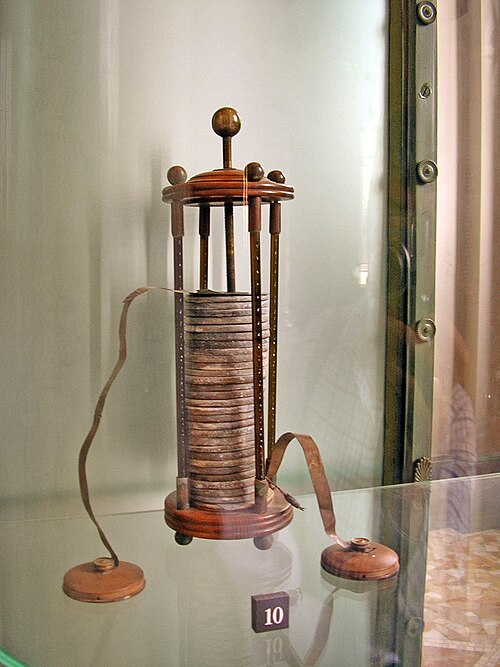
\includegraphics[width=\linewidth]{images/book3/volta-pile.jpg}
\end{minipage}\hfill
\begin{minipage}[t]{0.69\linewidth}
\vspace{0pt}
In 1800 Alessandro Volta described a column of discs of two different metals,
zinc and copper or silver, separated by cloth soaked in brine: the first
source of a steady electric current. Within weeks others used it to decompose
water, and within a decade Humphry Davy had isolated sodium and potassium by
\omterm{def:b2:batteries-electrolysis:electrolysis}{electrolysis} of their molten hydroxides with a large pile. The photograph shows
one of Volta's own piles. (Photograph: GuidoB, CC BY-SA 3.0, Wikimedia
Commons.)
\end{minipage}
\end{history}

\section{Fuel cells}

\begin{definition}[Fuel cell]\label{def:b2:batteries-electrolysis:fuel-cell}
A \emph{fuel cell}\index{fuel cell} is a cell whose reagents, a fuel and an
oxidant (usually the oxygen of the air), are fed continuously to its
electrodes and whose products are removed, so that it delivers current as long
as it is supplied.
\end{definition}

In the proton-exchange membrane cell of the bus of
\cref{ch:b2:cell-thermodynamics}, hydrogen is oxidised on a platinum catalyst,
\ce{H2 -> 2H+ + 2e-}, protons cross a thin acidic polymer membrane, and oxygen is
reduced on the other side, \ce{O2 + 4H+ + 4e- -> 2H2O}. The oxidation of hydrogen
on platinum is a \omterm{def:b2:current-potential-curves:fast-slow}{fast system}; the reduction of oxygen is slow on every
electrode. Most of the voltage lost between the \qty{1.23}{V} of the reversible
cell and the working voltage is the \omterm{def:b2:current-potential-curves:overpotential}{overpotential} of the oxygen electrode,
the rest the resistance of the membrane and, at high current, the supply of
oxygen to the catalyst (a \omterm{def:b2:current-potential-curves:limiting-current}{limiting current}).

\section{Electrolysis}

\begin{definition}[Electrolysis]\label{def:b2:batteries-electrolysis:electrolysis}
An \emph{electrolysis}\index{electrolysis} is a non-spontaneous redox reaction
forced by a current supplied by an external generator; the cell in which it
takes place is an \emph{electrolyser}\index{electrolyser}. The anode, where the
oxidation occurs, is connected to the positive pole of the generator.
\end{definition}

\begin{proposition}[Thermodynamic minimum voltage]\label{prop:b2:batteries-electrolysis:minimum-voltage}
An \omterm{def:b2:batteries-electrolysis:electrolysis}{electrolysis} whose reaction has $\Delta_r G > 0$ requires a voltage of at
least $\Delta_r G/(nF)$.
\end{proposition}

\begin{proof}
The generator supplies the work $nFU$ per mole of reaction; by
\cref{thm:b2:cell-thermodynamics:delta-g-nfe} applied to the reverse reaction, the
electrical work received must be at least $\Delta_r G$.
\end{proof}

\begin{proposition}[Voltage of an electrolyser]\label{prop:b2:batteries-electrolysis:electrolysis-voltage}
An \omterm{def:b2:batteries-electrolysis:electrolysis}{electrolyser} passing a current $I$ needs
\[
  U = (E_a - E_c) + \eta_a + |\eta_c| + rI ,
\]
with $E_a$, $E_c$ the equilibrium potentials of the anode and cathode couples
($E_a - E_c = \Delta_r G/(nF)$), $\eta_a$, $\eta_c$ their \omterm{def:b2:current-potential-curves:overpotential}{overpotentials} at that
current and $r$ the resistance between the electrodes.
\end{proposition}

\begin{proof}
As for a cell, the same current is anodic at the anode, at potential $E_a +
\eta_a$, and cathodic at the cathode, at $E_c + \eta_c$; the generator must also
drive it through the electrolyte, adding $rI$.
\end{proof}

\begin{method}[Predicting an electrolysis]\label{met:b2:batteries-electrolysis:predict-electrolysis}
\begin{enumerate}
  \item List every species that can be oxidised at the anode (including the
        anode metal and the solvent) and every species that can be reduced at
        the cathode (including the solvent).
  \item Draw their \omterm{def:b2:current-potential-curves:ie-curve}{current--potential curves} on the electrode materials used.
  \item As the voltage is raised, the first anodic curve and the first cathodic
        curve reached give the reactions; at larger currents, the next ones add
        theirs.
\end{enumerate}
\end{method}

\begin{definition}[Faradaic efficiency]\label{def:b2:batteries-electrolysis:faradaic-efficiency}
The \emph{faradaic efficiency}\index{faradaic efficiency} $\eta_F$ of an
\omterm{def:b2:batteries-electrolysis:electrolysis}{electrolysis} is the fraction of the charge passed that produces the wanted
product. Its \emph{specific energy consumption}\index{specific energy consumption}
is the electrical energy used per unit mass of product.
\end{definition}

\begin{proposition}[Faraday's law]\label{prop:b2:batteries-electrolysis:faraday-mass}
A current $I$ passed for a time $t$ with \omterm{def:b2:batteries-electrolysis:faradaic-efficiency}{faradaic efficiency} $\eta_F$ produces a
mass $m = \eta_F MIt/(nF)$ of a product of molar mass $M$ formed with $n$
electrons per mole.
\end{proposition}

\begin{proof}
The charge $It$, of which $\eta_F It$ forms the product, corresponds by
\cref{prop:b2:cell-thermodynamics:charge} to $\eta_F It/(nF)$ moles.
\end{proof}

\begin{proposition}[Energy per kilogram]\label{prop:b2:batteries-electrolysis:energy}
At a voltage $U$ and \omterm{def:b2:batteries-electrolysis:faradaic-efficiency}{faradaic efficiency} $\eta_F$, the \omterm{def:b2:batteries-electrolysis:faradaic-efficiency}{specific energy
consumption} is $w = nFU/(\eta_F M)$.
\end{proposition}

\begin{proof}
The energy is $UIt$ and the mass $\eta_F MIt/(nF)$; divide.
\end{proof}

\section{Industrial electrolyses}

\paragraph{Zinc.} Most zinc is won by \omterm{def:b2:batteries-electrolysis:electrolysis}{electrolysis} of the acidic zinc sulfate
solution of \cref{ch:b2:ellingham}. Zinc is deposited on the cathode although
\ce{H+} is the stronger oxidant: on zinc the reduction of \ce{H+} is very slow,
and the zinc wave is reached first; the anode gives off oxygen.

\begin{omfigure}
\begin{tikzpicture}
\begin{axis}[omie, width=0.82\linewidth, height=5.6cm, xmin=-1.6, xmax=2.4,
  ymin=-2.4, ymax=2.4, xlabel={$E$ (V)}, ylabel={$i$}, clip=true, clip mode=individual]
\addplot[omcathodic] table[x=E, y=i] {figdata/out/bachelor-2-ie-curves-g-cath.dat};
\addplot[omanodic] table[x=E, y=i] {figdata/out/bachelor-2-ie-curves-g-an.dat};
\draw[densely dotted] (axis cs:-0.76,-2.2) -- (axis cs:-0.76,0.4);
\draw[densely dotted] (axis cs:0,-2.2) -- (axis cs:0,0.4);
\node[font=\scriptsize, anchor=south] at (axis cs:-0.76,0.4) {$-0.76$};
\node[font=\scriptsize, anchor=south east] at (axis cs:-0.02,0.4) {$0$};
\node[font=\scriptsize, omDef, anchor=north west, align=left] at (axis cs:-0.7,-1.05) {\ce{Zn^2+} $\to$ \ce{Zn},\\ plateau};
\node[font=\scriptsize, omDef, anchor=east, align=right] at (axis cs:-1.32,-0.9) {\ce{H+} $\to$ \ce{H2}\\ on Zn};
\node[font=\scriptsize, omThm, anchor=east] at (axis cs:1.85,1.6) {\ce{H2O} $\to$ \ce{O2}};
\node[font=\scriptsize, gray, align=center] at (axis cs:-0.38,-0.5) {no \ce{H2}\\ on zinc here};
\end{axis}
\end{tikzpicture}

{\small \omterm{def:b2:batteries-electrolysis:electrolysis}{Electrolysis} of an acidic zinc sulfate solution with a zinc cathode
(model curves). Although the \ce{H+}/\ce{H2} couple ($\qty{0}{V}$) lies above
\ce{Zn^2+}/\ce{Zn} ($\qty{-0.76}{V}$), the reduction of \ce{H+} on zinc does
not start before about \qty{-1.1}{V}: between, zinc is deposited alone. At the
anode, water is oxidised to oxygen.}
\end{omfigure}

\paragraph{Chlorine and sodium hydroxide.} Brine is electrolysed in a cell
divided by a membrane that lets only cations through. At the anode chloride is
oxidised, \ce{2Cl- -> Cl2 + 2e-}; at the cathode water is reduced, \ce{2H2O +
2e- -> H2 + 2OH-}; sodium ions cross the membrane to balance the charge, and a
sodium hydroxide solution leaves the cathode side, free of chloride. The
thermodynamic minimum is $\Delta_r G/(2F) = \qty{2.19}{V}$ for \ce{2Cl- + 2H2O -> Cl2 +
H2 + 2OH-} in standard conditions. Chlorine forms at the anode rather than
oxygen, though the \ce{O2}/\ce{H2O} couple lies lower: the oxidation of water
is the slower of the two on the anode materials used.
% ledger: dfg:OH-_ao, dfg:Cl-_ao, dfg:H2O_l

\begin{omfigure}
\begin{tikzpicture}[font=\small, >={Stealth}]
  \draw[thick] (0,0) rectangle (6,3.4);
  \draw[thick, dashed, omProp] (3,0) -- (3,3.4);
  \fill[black!30] (0.4,0.3) rectangle (0.7,3.0);
  \fill[black!50] (5.3,0.3) rectangle (5.6,3.0);
  \node[font=\scriptsize] at (0.55,3.3) {$+$};
  \node[font=\scriptsize] at (5.45,3.3) {$-$};
  \node[font=\scriptsize, align=center] at (1.85,1.9) {brine\\ \ce{2Cl-} $\to$\\ \ce{Cl2 + 2e-}};
  \node[font=\scriptsize, align=center] at (4.2,1.9) {\ce{NaOH}\\ solution\\ \ce{2H2O + 2e-} $\to$\\ \ce{H2 + 2OH-}};
  \draw[->, thick, omDef] (2.6,0.8) -- (3.4,0.8) node[pos=0.1, above, font=\scriptsize] {\ce{Na+}};
  \draw[->, thick] (1.0,3.4) -- (1.0,4.0) node[above] {\ce{Cl2}};
  \draw[->, thick] (5.0,3.4) -- (5.0,4.0) node[above] {\ce{H2}};
  \draw[->, thick] (-0.8,0.6) -- (0,0.6) node[pos=0, left] {brine in};
  \draw[->, thick] (6,0.6) -- (6.8,0.6) node[right] {\ce{NaOH} out};
  \node[font=\scriptsize, omProp, anchor=north] at (3,-0.05) {cation-exchange membrane};
\end{tikzpicture}

{\small A membrane chlor-alkali cell, schematic. Only sodium ions cross the
membrane, so the hydroxide formed at the cathode does not meet the chlorine.}
\end{omfigure}

\paragraph{Aluminium.} Aluminium oxide is dissolved in molten cryolite,
\ce{Na3AlF6}, which melts far lower than alumina, and electrolysed between a
carbon cathode, on which liquid aluminium collects, and carbon anodes that
burn away as carbon dioxide (Hall--Héroult process):
\[
  \ce{2Al2O3 + 3C -> 4Al + 3CO2} .
\]
The thermodynamic minimum near \qty{1250}{K} is about \qty{1.18}{V}
(\cref{pb:b2:batteries-electrolysis:1}); the cell of that problem works at three
and a half times as much, the excess turned into the heat that keeps the bath
molten.

\begin{omfigure}
\begin{tikzpicture}[font=\small, >={Stealth}]
  \draw[thick, fill=black!12] (0,0) rectangle (7,3.2);
  \fill[black!45] (0.3,0.3) rectangle (6.7,0.8);
  \fill[gray!35] (0.3,0.8) rectangle (6.7,1.4);
  \fill[orange!30] (0.3,1.4) rectangle (6.7,2.5);
  \foreach \x in {1.0,3.0,5.0} {
    \fill[black!75] (\x,1.75) rectangle (\x+1.0,3.6);
    \draw[thick] (\x+0.5,3.6) -- (\x+0.5,4.2);
  }
  \draw[thick] (1.5,4.2) -- (5.5,4.2) node[right] {$+$};
  \node[font=\scriptsize, align=left, anchor=west] at (7.3,2.6) {carbon anodes, burnt to \ce{CO2}};
  \node[font=\scriptsize, align=left, anchor=west] at (7.3,1.95) {molten cryolite + dissolved \ce{Al2O3}};
  \node[font=\scriptsize, align=left, anchor=west] at (7.3,1.1) {liquid aluminium (cathode)};
  \node[font=\scriptsize, align=left, anchor=west] at (7.3,0.55) {carbon cathode block, $-$};
  \draw[densely dotted] (6.7,2.6) -- (7.3,2.6) (6.7,1.95) -- (7.3,1.95) (6.7,1.1) -- (7.3,1.1) (6.7,0.55) -- (7.3,0.55);
\end{tikzpicture}

{\small A Hall--Héroult cell, cross-section, schematic. Aluminium is reduced
at the surface of the liquid metal pool, which acts as cathode; the oxide ions
discharge on the carbon anodes, which they burn to carbon dioxide.}
\end{omfigure}

\begin{history}[Hall and Héroult, 1886]
\begin{minipage}[t]{0.18\linewidth}
\vspace{0pt}
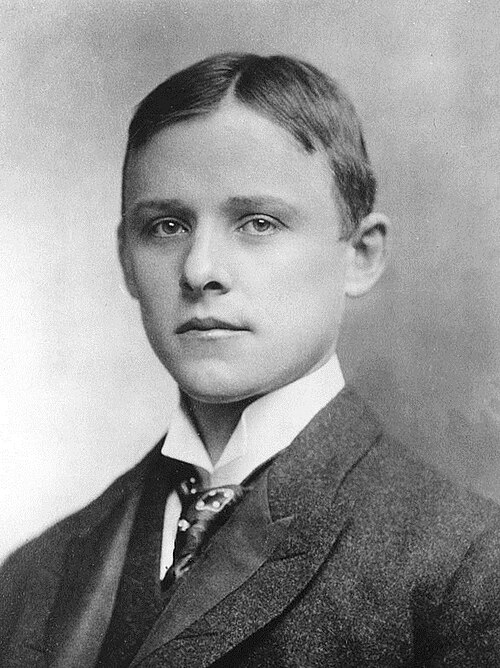
\includegraphics[width=\linewidth]{images/book3/hall.jpg}
\end{minipage}\hspace{0.02\linewidth}%
\begin{minipage}[t]{0.18\linewidth}
\vspace{0pt}
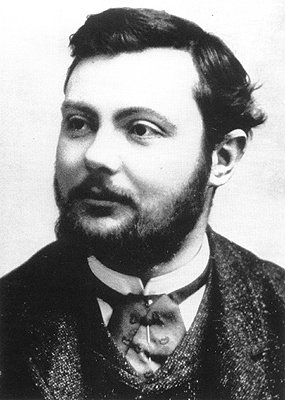
\includegraphics[width=\linewidth]{images/book3/heroult.jpg}
\end{minipage}\hfill
\begin{minipage}[t]{0.58\linewidth}
\vspace{0pt}
In 1886, at the age of twenty-two or twenty-three, Charles Martin Hall and
Paul Héroult, on the two sides of the Atlantic, found independently that alumina
dissolves in molten cryolite and can be electrolysed there. Aluminium, until
then a precious metal made by reducing its chloride with sodium, became the
cheapest of the light metals once electricity could be generated in bulk.
(Portraits: Hall, about 1880s, unknown author, public domain; Héroult,
public domain; Wikimedia Commons.)
\end{minipage}
\end{history}

\paragraph{Sodium.} Sodium cannot be deposited from water, which it reduces.
It is made by \omterm{def:b2:batteries-electrolysis:electrolysis}{electrolysis} of molten sodium chloride, its melting point
lowered by an added salt (a \omterm{def:b2:solid-liquid-diagrams:eutectic}{eutectic mixture}, \cref{ch:b2:solid-liquid-diagrams}),
with chlorine as by-product. At \qty{1100}{K}, $\Delta_f G^\circ(\ce{NaCl}, \text{l}) =
\qty{-310.7}{kJ/mol}$: the minimum voltage is \qty{3.22}{V}.
% ledger: janafG:NaCl.1100

\section{Exercises}

\begin{exercise}[$\star$]\label{exo:b2:batteries-electrolysis:1}
On the zinc-in-acid figure, read the \omterm{def:b2:batteries-electrolysis:mixed-potential}{mixed potential} and the current of zinc
alone and of zinc touching copper (model units), and say which dissolves
faster.
\end{exercise}

\begin{exercise}[$\star$]\label{exo:b2:batteries-electrolysis:2}
What mass of zinc is deposited in one hour by a current of \qty{500}{A} with a
\omterm{def:b2:batteries-electrolysis:faradaic-efficiency}{faradaic efficiency} of 100~\%?
\end{exercise}

\begin{exercise}[$\star$]\label{exo:b2:batteries-electrolysis:3}
Compute the standard voltage of the lead--acid \omterm{def:b2:batteries-electrolysis:battery}{accumulator} from the Gibbs
energies of formation given in the chapter, and the number of cells in a
\qty{12}{V} car battery.
\end{exercise}

\begin{exercise}[$\star$]\label{exo:b2:batteries-electrolysis:4}
What charge, in ampere-hours, can one gram of lithium deliver if it is all
oxidised to \ce{Li+}?
\end{exercise}

\begin{exercise}[$\star\star$]\label{exo:b2:batteries-electrolysis:5}
A copper refining cell passes \qty{200}{A} for \qty{24}{h} and deposits
\qty{5.50}{kg} of copper. Compute the \omterm{def:b2:batteries-electrolysis:faradaic-efficiency}{faradaic efficiency}.
\end{exercise}

\begin{exercise}[$\star\star$]\label{exo:b2:batteries-electrolysis:6}
A zinc electrowinning cell works at \qty{3.3}{V} with a \omterm{def:b2:batteries-electrolysis:faradaic-efficiency}{faradaic efficiency} of
90~\% (exercise data). Compute the electrical energy per kilogram of zinc.
\end{exercise}

\begin{exercise}[$\star\star$]\label{exo:b2:batteries-electrolysis:7}
A battery gives \qty{1.55}{V} at \qty{0.10}{A} and \qty{1.40}{V} at \qty{0.60}{A}.
Assuming the \omterm{def:b2:current-potential-curves:overpotential}{overpotentials} negligible, find its internal resistance and its
voltage with no current.
\end{exercise}

\begin{exercise}[$\star\star$]\label{exo:b2:batteries-electrolysis:8}
Brine is electrolysed in the membrane cell. Write the electrode reactions,
compute the minimum voltage, and explain why the products must be kept
apart.
\end{exercise}

\begin{exercise}[$\star\star$]\label{exo:b2:batteries-electrolysis:9}
Compute the minimum voltage for the \omterm{def:b2:batteries-electrolysis:electrolysis}{electrolysis} of molten sodium chloride at
\qty{1100}{K} and the minimum energy per kilogram of sodium.
\end{exercise}

\begin{exercise}[$\star\star\star$]\label{exo:b2:batteries-electrolysis:10}
Using \omterm{def:b2:current-potential-curves:ie-curve}{current--potential curves}, explain why zinc can be plated from an acidic
bath on a zinc cathode, and predict what would happen on a platinum cathode at
the start of the plating.
\end{exercise}

\begin{exercise}[$\star\star\star$]\label{exo:b2:batteries-electrolysis:11}
From $\Delta_f G^\circ$ at \qty{1100}{K} and \qty{1300}{K} ($\ce{Al2O3}$: $-1328.3$ and
$-1262.3$; $\ce{CO2}$: $-396.0$ and $-396.2$ \unit{kJ/mol}), compute the minimum
voltage of the Hall--Héroult cell at \qty{1250}{K}, and compare it with an
inert anode on which oxygen would be released.
\end{exercise}

\begin{exercise}[$\star\star\star$]\label{exo:b2:batteries-electrolysis:12}
Electricity is stored by electrolysing water at \qty{1.80}{V} and recovered in a
\omterm{def:b2:batteries-electrolysis:fuel-cell}{fuel cell} at \qty{0.70}{V}, both with a \omterm{def:b2:batteries-electrolysis:faradaic-efficiency}{faradaic efficiency} of 100~\%. Compute the
round-trip efficiency and explain where the energy goes.
\end{exercise}

\section{Problem: One Tonne of Aluminium}

\begin{problem}[{Weekend problem --- the reaction of the Hall--Héroult cell
and its minimum voltage, the charge and time to make a tonne of aluminium,
the energy used, and the carbon burnt}]
\label{pb:b2:batteries-electrolysis:1}
Data: JANAF Gibbs energies of formation at \qty{1100}{K} and \qty{1300}{K}
(\unit{kJ/mol}): \ce{Al2O3} $-1328.3$, $-1262.3$; \ce{CO2} $-396.0$, $-396.2$. Cell
(exercise data): current \qty{300}{kA}, voltage \qty{4.1}{V}, \omterm{def:b2:batteries-electrolysis:faradaic-efficiency}{faradaic efficiency}
94~\%, bath near \qty{1250}{K}. Molar masses (\unit{g/mol}): Al 26.982, C 12.011,
O 15.999. Heat to bring aluminium from \qty{298}{K} to liquid at its melting
point: \qty{28.69}{kJ/mol}.
% ledger: janafG:Al2O3.1100, janafG:Al2O3.1300, janafG:CO2.1100, janafG:CO2.1300, aw:Al, aw:C, aw:O, hT:Al_l.933, const:F

\medskip
\noindent\textbf{Part I --- The minimum voltage.}
\begin{enumerate}
  \item Give the oxidation numbers of aluminium, oxygen and carbon in the
        reactants and products.
  \item Write the cathode and anode half-reactions, with the oxide ion
        \ce{O^2-} carried by the molten bath.
  \item Write the overall reaction and the number $n$ of electrons exchanged.
  \item Interpolate $\Delta_f G^\circ$ of \ce{Al2O3} and \ce{CO2} at \qty{1250}{K}.
  \item Compute $\Delta_r G^\circ$ at \qty{1250}{K}.
  \item Deduce the minimum voltage.
  \item Compute the minimum voltage with an inert anode,
        \ce{2Al2O3 -> 4Al + 3O2}, and explain the role of the carbon.
\end{enumerate}

\medskip
\noindent\textbf{Part II --- Charge and time.}
\begin{enumerate}[resume]
  \item What amount of aluminium is in one tonne?
  \item What charge would it need with a \omterm{def:b2:batteries-electrolysis:faradaic-efficiency}{faradaic efficiency} of 100~\%?
  \item What charge is actually passed?
  \item How long does one cell take to make a tonne?
  \item What mass of aluminium does one cell make per day?
  \item Suggest where the lost 6~\% of the charge goes.
\end{enumerate}

\medskip
\noindent\textbf{Part III --- Energy.}
\begin{enumerate}[resume]
  \item Compute the electrical energy per tonne.
  \item Express it in \unit{kW.h} per kilogram.
  \item Compute the minimum energy per kilogram, at the minimum voltage and
        100~\% efficiency.
  \item Where does the rest of the energy go, and why is it not wasted
        entirely?
  \item Compute the electrical power of one cell.
  \item Compute the heat needed to remelt one kilogram of scrap, in
        \unit{kW.h}, and compare.
  \item What fraction of the working voltage is the thermodynamic minimum?
\end{enumerate}

\medskip
\noindent\textbf{Part IV --- Carbon.}
\begin{enumerate}[resume]
  \item Compute the mass of carbon burnt per tonne of aluminium according to the
        equation.
  \item Compute the mass of carbon dioxide released by the anodes per tonne.
  \item Real cells burn more carbon than that. Suggest two reasons.
  \item Express the anode \ce{CO2} per kilogram of aluminium.
  \item What would an inert anode change for the voltage and for the gas
        released?
  \item State the electrical energy per kilogram of aluminium.
\end{enumerate}
\end{problem}
